\chapter{Software Qualität}

\section{Einführung}

Im Themenbereich der Software Qualität werden wünschenswerte Attribute eines Software-Produkts beschrieben. Die Qualitätssicherung muss über den gesamten Software-Lebenszyklus berücksichtigt werden - von der Analyse bis zum Betrieb. Interessant ist die Kostenverteilung nach Böhm mit und ohne Wartung von Software auf Abbildung \ref{fig:kostenverteilung-sw-entwicklung-nach-boehm}.

\begin{figure}[h!]
\centering
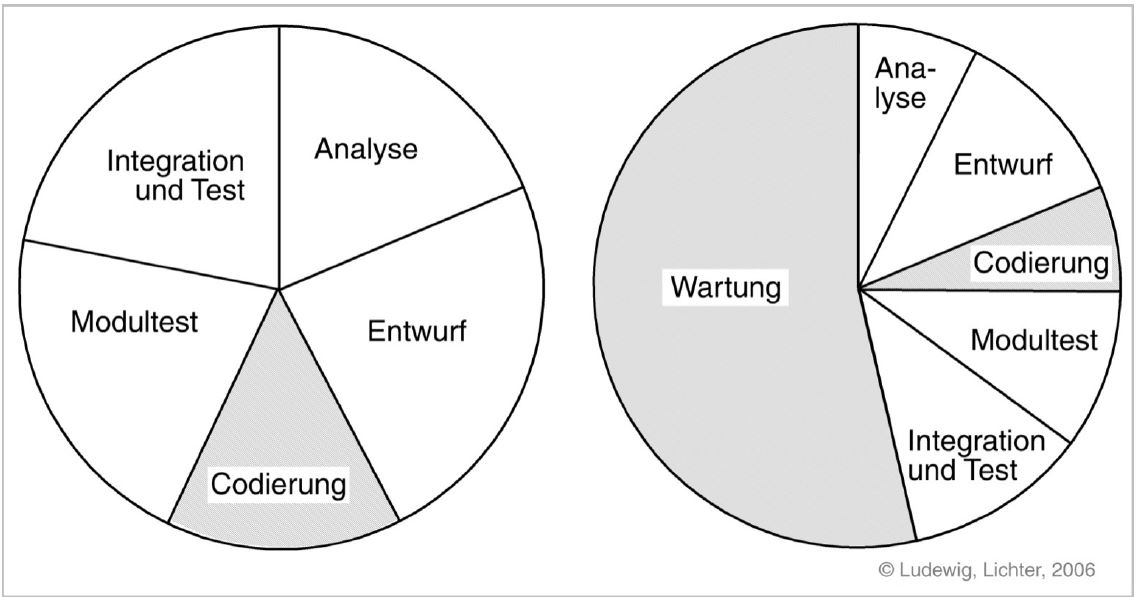
\includegraphics[width=0.8\linewidth]{fig/kostenverteilung-sw-entwicklung-nach-boehm}
\caption{Kostenverteilung nach Böhm. Ohne Wartung (links), mit Wartung (rechts)}
\label{fig:kostenverteilung-sw-entwicklung-nach-boehm}
\end{figure}

In der Software-Entwicklung läuft teilweise vieles falsch. Neben zu optimistischen Plänen und unrealistischen Erwartungen gilt auch \emph{shortchanged quality assurance} als Problem. Mit letzterem ist gemeint, dass wenn ein Projekt in Verzug kommt, dass das auf Kosten der Qualitätssicherenden-Massnahmen geht. Es werden keine Code-Reviews gemacht, die Anzahl der Unit-Test nimmt nicht mehr zu, es wird noch nicht mal mehr Software-Design betrieben. Im Fokus steht nur noch Codezeilen / Zeiteinheit. Als Resultat hat man zwar ein \emph{feature complete}, aber fehlerhaftes Software-Produkt. Ein Tag eingesparte QA in einer früheren Entwicklungsphase kostet 3-10 Tage Entwicklungs-Aufwand in einer späteren Phase.

Es gibt unterschiedliche Interessenten für gute Software Qualität. Dies sind die Entwickler, die Sponsoren und letztendlich die Kunden. Kategorisiert werden drei unterschiedliche Qualitäten: Process Quality, Structural Quality, Functional Quality. Ein wichtiger Fokus liegt auf der Code Qualität. Die Bewegung \emph{Clean Code} bringt viele Ansätze ins Spiel, welche die Qualität des Codes erhöhen.

Wenn Entwickler sich in ein Projekt einarbeiten, ist ein erster Anhaltspunkt die Qualität der Software:
\begin{description}
	\item[Testbarkeit] Ist die Software so organisiert, dass sie einfach getestet werden kann?
	
	\item[Wartbarkeit] Wie leicht kann neue Code hinzugefügt oder vorhandener Code geändert werden, ohne dass Fehler verursacht werden?
	
	\item[Verständlichkeit] Ist der Code lesbar? Ist die Komplexität beherrschbar? Ist der Code unnötig komplex?
\end{description}

\subsection{Gerichtliche Aspekte}
Wichtig zu wissen ist, dass nicht nur die Code Qualität ausschlaggebend ist. Vor einem Gericht spielt die gesamte Software Qualität, was den gesamten Software-Entwicklungsprozess berücksichtigt, eine Rolle. Bei einem Fallbeispiel hat ein Gericht unter dem Punkt Software Qualität folgende Aspekte angeschaut:

\begin{itemize}
	\item Dokumentation
	\item Projektmanagement
	\item Architektur
	\item Requirements Engeneering
	\item Testkonzept
	\item Vorgehensmodell
\end{itemize}

Zudem wurde auch der Code angeschaut:
\begin{itemize}
	\item Globale Variabeln / viele verstreute Zugriffe
	\item Design Prinzipien
	\item Redundanter Code
	\item Fehlerbehandlung
	\item Fehlende / unklare Anforderungen
	\item Keine einheitliche Namensgebung
\end{itemize}

\subsection{Metriken}
Metriken stellen die quantitative Basis für die Entwicklung und Validierung von Modellen des Softwareentwicklungsprozesses dar. Mit anderen Worten, sie sind die Masse für Software Produkte und den dazugehörigen Entwicklungsprozess (Produkt = Source + Objektcode + Dokumentation). Man will eine \emph{Vorhersage} von Produktparametern.

Es gibt unterschiedliche Skalen:
\begin{figure}[h!]
\centering
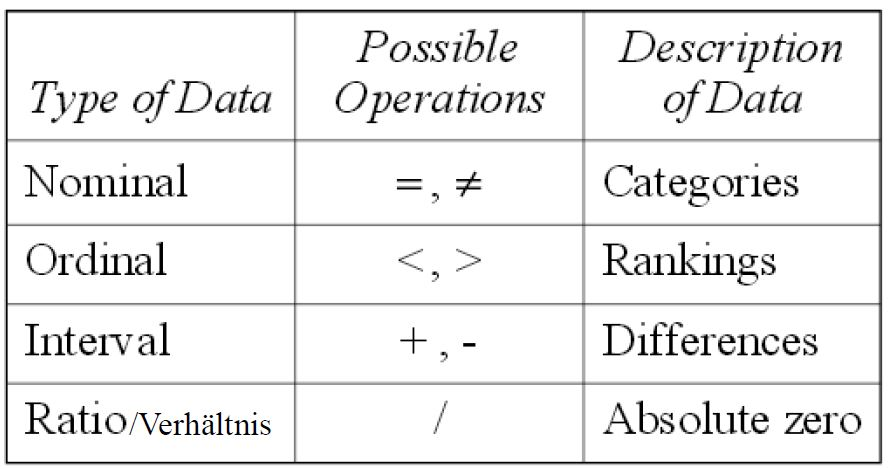
\includegraphics[width=0.7\linewidth]{fig/software-quality-skalen}
\caption{Skalen}
\label{fig:software-quality-skalen}
\end{figure}

\begin{description}
	\item[Nominalskala] Einordnung in verschiedene Kategorien, ohne dass eine Ordnung der Kategorien möglich ist. Beispiel: Der verwendete Vorgehensprozess ist SCRUM, RUP, HERMES, V-Modell, HTAgil, Wasserfall oder XP. Die Skalierung muss vollständig und ausschliessend sein, d. h., ein Element kann nur genau zu einer Kategorie gehören und die Kategorien müssen alle möglichen Elemente abdecken
	
	\item[Ordinalskala] Einordnung in Kategorien, die eine strikte Ordnung aufweisen, d.h., eine Kategorie ist besser oder > als die andere. Beispiel: Die Kundenzufriedenheit war sehr gut, gut, genügend oder ungenügend. Jede Kategorie muss klar definierte Kriterien haben, die festlegen, ob ein Artifakt zu dieser Kategorie gehört (Objektivität der Metrik sonst nicht gegeben). Die Abstände zwischen den Kategorien können nicht verglichen werden.
	
	\item[Intervallskala] Den einzelnen Mess-Ergebnissen können Zahlwerte zugeordnet werden und die Ergebnisse können direkt numerisch verglichen werden. Beispiel: Zyklomatische Komplexität einer Anweisung A ist 6, einer Anweisung B ist 2. A hat eine um 4 höhere Komplexität, aber wir können nicht sagen, dass die Komplexität von A umd dreimal höher ist als bei B. Es gibt keinen oder nur einen willkürlichen Nullwert. Es ist nicht sinnvoll, Werte zueinander ins Verhältnis zu setzen.
	
	\item[Verhältnisskala] Wie die Intervallskala, aber es existiert ein objektiv bestimmbarer Nullwert. Beispiel: durchschnittliche Anzahl Fehler für Produkt A = 5 Fehler/KLOC, Produkt B = 2.5 Fehler/KLOC. Fehlerrate für A ist doppelt so hoch wie für B. Werte können sinnvoll zueinander ins Verhältnis gesetzt werden.
\end{description} 

Beispiel-Metriken:
\begin{description}
	\item[Efferent Couplings] \textit{It measures the number of data types a class knows about.}. Die Anzahl Klassen die ein einzelne Klasse kennt.
	
	\item[Cyclomatic Complexity] Anzahl der binären Verzweigungen. Jede Methode hat einen Grundwert von 1. +1 für jedes if, while, do, for, ?:, catch, case. +1 für jedes Vorkommen der Operatoren \&\& oder ||.
	
	\item[Lack of Cohesion nach Henderson-Sellers] Wird überall anders berechnet. Beschreibt den Zusammenhalt von Methoden in der betrachteten Klasse. Wir brauchen bei der Berechnung die Information darüber, welche Methoden auf welche Instanzvariabeln zugreifen.
\end{description}

Das SQALE Rating bewertet ein Software-Artefakt indem es den geschätzten Aufwand für die Beseitigung eines Mangels in Bezug zum gesamten Entwicklungsaufwand ins Verhältnis setzt. Beispiel: Kosten in WorkUnits (WU) und Grösse in KLOC (1000 Zeilen Code) 1 KLOC erfordert 100 WU. Entwicklungskosten: 5 KLOC = 500 WU. Maintainability Aufwand: 15 WU. 15/500 = 3% = C.

\begin{figure}[h!]
\centering
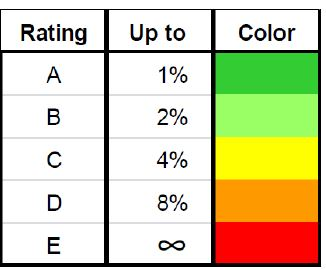
\includegraphics[width=0.1\linewidth]{fig/sqale-rating}
\caption{SQALE Rating}
\label{fig:sqale-rating}
\end{figure}

\section{Refactoring}

Beim Refactoring wir die interne Struktur eines Softwaresystems verbessert, ohne dabei die Funktionalität zu verändern. Dadurch kann man schlechtes Design in schön strukturierten Code umwandeln. Um keine neuen Fehler in den Code einzubauen, braucht es ein diszipliniertes Vorgehen. Beim Refactoring macht man kleine einfache Schritte, die zusammengefasst eine positiven Einfluss auf das Design haben. Nochmals es wird das Design verbessert, indem man den Code verbessert.

Bei vielen Softwareprojekten wird die Software zuerst designt und dann ausprogrammiert. Das funktioniert am Anfang auch recht gut, aber mit der Zeit ändert sich der Code und die Qualität nimmt ab. Hier hilft ein Refactoring, um die Codequalität trotzdem hoch zu halten. Man lernt während dem Bauen des Systems, wie man das Design verbessern kann und den Code so leichter verständlich und veränderbar macht. Ein ähnlicher Weg geht auch Scrum, wobei da eher die Anforderungen im Vordergrund stehen. Mit diesem Wissen kann das Twin Peak Modell von Nuseibeh um einen weiteren Peak für das Design erweitert werden (siehe Abbildung \ref{fig:twin-peaks-1}).

\begin{figure}
\centering
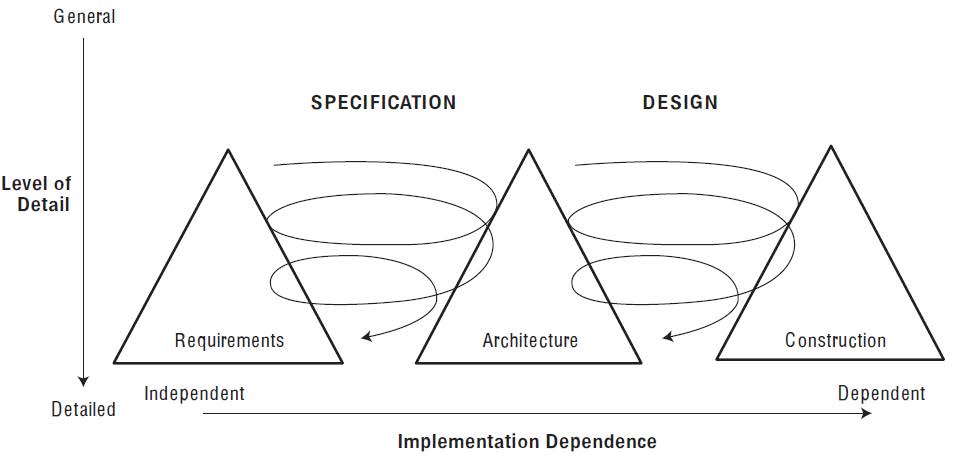
\includegraphics[width=0.7\linewidth]{fig/twin-peaks}
\caption{Twin Peaks}
\label{fig:twin-peaks-1}
\end{figure}

Ein Rafactoring sollte bei folgenden Szenarien durchgeführt werden:
\begin{itemize}
	\item Bevor neue Funktionalität zu bestehender Software hinzugefügt wird
	\item Beim Einarbeiten in unbekannte Software (Code Reviews)
	\item Zur Isolierung und Identifikation von Fehlern
	\item Wenn sich Anzeichen für schlechte Qualität häufen
	\item Zur Verbesserung der Entwicklungsproduktivität
\end{itemize}
Mangelnde Codequalität drückt sich durch folgende Anzeichen aus:
\begin{itemize}
	\item Viele globale Variablen
	\item Verstreute Zugriffe auf diese Variablen
	\item Schlecht verständliche Methoden- und Variablennamen
	\item Fehlende und schlecht verständliche Kommentare
	\item Fehlerbehandlung nicht explizit vorhanden
	\item Kopierter / redundanter Code
	\item Bad Smells (Kent Beck)
\end{itemize}
Es gibt folgende Bad Smells die eher auf eine Klasse angewendet werden:
\begin{description}
	\item Duplicated Code
	\item Long Method
	\item Large Class
	\item Long Parameter List
	\item Feature Envy
	\item Switch Statements
	\item Inappropriate Intimacy
	\item Lazy Class
	\item Data Class
	\item Message Chains
	\item Middle Man
	\item Comments
\end{description}
Die folgenden Bad Smells beziehen sich eher auf das Gesamtsystem:
\begin{itemize}
	\item Divergent Change
	\item Shotgun Surgery
	\item Data Clumps
	\item Primitive Obsession
	\item Parallel Inheritance Hierarchies
	\item Speculative Generality
	\item Temporary Field
	\item Alternative Classes with Different Interfaces
	\item Incomplete Library Class
	\item Refused Bequest
\end{itemize}
Aufgrund dieser Bad Smells wurde von Martin Fowler ein Refactoring-Katalog erstellt, welcher den Fokus auf objektorientierte Programmierung richtet (keine Unterstützung für parallele Programme, verteilte Systeme usw.). Für diese Refactorings gibt es auch eine gute Toolunterstützung. 